
Most of the content in this chapter appears in the article
\emph{\textsc{PresQ}: Discovery of Multidimensional Equally-Distributed Dependencies via Quasi-Cliques on Hypergraphs}~\cite{AlvarezAyllonPresQ2022},
published on \emph{IEEE Transactions on Emerging Topics in Computing}.

\medskip

\PresQ is a statistically robust algorithm for finding \glspl{EDD}, as described
in definition~\ref{def:eqdist}.

Following the \emph{Engineering Design} process, \PresQ is the \emph{output} of
the \emph{embodiment design} phase of the design process, and the present chapter
is its documentation.
In section~\ref{sec:presq_definitions}, we list the set of rules needed to be able
to define a search space for \glspl{EDD} and introduce the concepts of
hypergraph and quasi-clique. In section~\ref{sec:presq_inferring}, we propose
a novel algorithm based on quasi-cliques to infer common equally-distributed
multidimensional attributes.
In section~\ref{sec:presq_experiments}, we show experimental results
that prove that \PresQ successfully finds dependencies in a reasonable amount of time.
Finally, in section \ref{sec:presq_conclusions}, we compile the conclusions and
propose areas for further work.

\section{Definitions}
\label{sec:presq_definitions}

\subsection{Equally Distributed Dependencies}
\label{sec:edd}
An Inclusion Dependency exists if all combinations of
values from a given set of attributes in one relation are contained within
a set of attributes from another.
However, we will hardly ever find a strict
subset relation between two attributes in the real domain. Measurements may have associated uncertainty,
and even floating-point representation may vary (i.e. 32 vs 64 bits). It is generally a
flawed idea to compare floating-point numbers with strict equality.

Instead, we can use $R.X \eqdist S.Y$ as an approximation, meaning that the two sets of
attributes are equally distributed. This relation is, unlike the subset relation, symmetrical.

Following the parallelism with \gls{IND} finding, we say that the dataset $d$ satisfies
the relation defined by equality of distribution $\eqdist$ when a statistical test
fails to reject the null hypothesis
\begin{equation}
    H_0: P(R[X]) = P(S[Y])
    \label{eq:eqdist}
\end{equation}
Three inference rules can be used to derive some additional \glspl{IND} from an already known
set of \glspl{IND}. They are defined using sets and subsets \cite{Casanova1984},
but they translate to the equality of distribution:

\begin{description}
    \item[Reflexivity] \hfill \\
        $R[X] \eqdist R[X]$
    \item[Permutation and projection] \hfill \\
        If $R[A_1,\dots,A_n] \eqdist S[B_1,\dots,B_n]$ then
        $R[A_{i_1},\dots,A_{i_m}] \eqdist S[B_{i_1},\dots,B_{i_m}]$ for each sequence
        $i_1,\dots,i_m$ of distinct integers from $\{1,\dots,n\}$
    \item[Transitivity] \hfill \\
        $ R[X] \eqdist S[Y] \land S[Y] \eqdist T[Z] \implies R[X] \eqdist T[Z]$
\end{description}

The reflexivity, permutation, and transitivity rules are well-known to hold
for $\eqdist$ \cite{randles1979introduction}.

%We have proven that the projection rule also holds, as is logical~\cite{Alvarez2021inference}.
For the projection, we need to prove that if two sets of random variables
$X_1,\dots,X_n$ and $Y_1,\dots,Y_n$ are equally distributed, so are
any of their possible sub-sequences.

\begin{proof}
Let $X'$ and $Y'$ be the sequences $X_1,\dots,X_m$ and $Y_1,\dots,Y_m$ with $m < n$.
Their corresponding  \gls{CDF} are just the \emph{marginal} \gls{CDF}:

\begin{equation}
\begin{split}
    F_{X_1,\dots,X_m}(x_1,\dots,x_m) = & F_{X_1,\dots,X_m,X_{m+1},X_n}(x_1,\dots,x_m,x_{m+1},\dots,x_n) \\
    F_{Y_1,\dots,Y_m}(y_1,\dots,y_m) =& F_{Y_1,\dots,Y_m,Y_{m+1},Y_n}(x_1,\dots,x_m,x_{m+1},\dots,x_n)\\
    & \forall (x_1,\dots,x_m) \in \mathbb{R}^m \textrm{ and } x_i \xrightarrow{} \infty \; \forall i > m
\end{split}
\end{equation}

By definition \ref{def:eqdist}, the right hand-side of both equations must be the same.
By transitivity, 

\begin{equation}
\begin{split}
    & F_{X_1,\dots,X_m}(x_1,\dots,x_m) = F_{Y_1,\dots,Y_m}(y_1,\dots,y_m) \\
    & \implies X_1,\dots,X_m \eqdist Y_1,\dots,Y_m
\end{split}
\end{equation}

\end{proof}

Thanks to the validity of these rules, particularly the permutation and projection,
we can use the specialization relation seen in definition \ref{def:specialization}
when dealing with distributions.

With these rules, we have defined the search space similar to the one from \gls{IND} discovery.
The last requirement is a property that allows the pruning of the
search space as illustrated in figure~\ref{fig:lattice}.

Let $I = R[X] \eqdist S[Y]$.
A dataset $d$ \emph{satisfies} $I$ iff  a statistical test fails to reject $H_0: P(R[X]) = P(S[Y])$
given a significance level $\alpha$.
This is denoted as $d \models I$.

\begin{property}
    Given $I_1 \prec I_2$:
    
    \label{prop:prob_spec}
    \begin{enumerate}
        \item If $d \models I_2$, then $d \models I_1$ (Accepting $H_{0_2}$ implies accepting $H_{0_1}$\footnotemark)
        \item $d \not\models I_1$ with a probability $\alpha$ when $d \models I_2$
            (Rejecting $H_{0_1}$ \emph{does not} imply the rejection of $H_{0_2}$)
    \end{enumerate}
\end{property}

\footnotetext{Strictly speaking, \emph{not rejecting} $H_{0_2}$ implies that we can not reject $H_{0_1}$.}

This property is similar to that proposed for \glspl{IND}~\cite{DeMarchi2002}, with the exception that even if $d \models I_2$, there is a probability to falsely reject $I_1$ bound by the significance level $\alpha$.

\begin{example}
    If we have two sets of $10$ attributes that are equally distributed, the number of
    3-dimensional projections (specializations) that must be equally distributed will be $\binom{10}{3} = 120$ .
    If we have a significance level of $\alpha = 0.1$, the expected number of
    falsely rejected 3-dimensional equalities is then $12$.
\end{example}

\subsection{Uniform n-Hypergraphs and quasi-cliques}

A hypergraph is a generalization of a graph where the edges may connect any number
of nodes.
It is defined as a pair $H = (V, E)$, with $V$ the set of nodes and $E$ the set of edges. An edge $e \in E$ is a set of distinct elements from $V$.

\begin{definition}
    \label{def:khypergraph}    
    Given the hypergraph $H = (V, E)$, $H$ is a \emph{n-hypergraph} iff
    all of its edges have size $n$.
\end{definition}

A clique or hyper-clique on a $n$-hypergraph $H = (V, E)$ is a set of nodes
$V' \subseteq V$ such that
every edge defined by the permutations of distinct $n$ nodes from $V'$ exists in $E$
\cite{koeller2003discovery}.

A quasi-clique or hyper-quasiclique (sometimes named pseudo-clique) is a generalization of a clique
where a given number of edges can be missing. The exact definition can be based
on the ratio of missing edges or based on the node degrees. Another option
is to combine both measures \cite{brunato2007effectively}, which is our preferred method.

We generalize the definition of quasi-cliques to $k$-uniform hypergraphs :

\begin{definition}
    \label{def:quasi_clique}
    Given a k-uniform hypergraph $(V,E)$, and two parameters $\lambda, \gamma \in [0,1]$
    the sub-graph $H'=(V',E')$ induced by a subset $V' \subseteq V$ is a
    $(\lambda-\gamma)$ quasi-clique iff:
    
    \begin{equation}
        |E'| \ge \gamma \cdot \binom{|V'|}{k}
        \label{eq:edge_hyperclique}
    \end{equation}
    
    \begin{equation}
        \forall v \in V': deg_{V'}(v) \ge \lambda \cdot \binom{|V'| - 1}{k - 1}
        \label{eq:deg_hyperclique}
    \end{equation}
    
    Where $deg_{V'}(v)$ represents the degree of $v$, and $E'$ is a subset of $E$ such that
    $\forall e \in E' : e \subseteq V'$
\end{definition}

In other words, condition~\ref{eq:edge_hyperclique} allows for some edges to be missing,
while condition~\ref{eq:deg_hyperclique} enforces a lower bound on the degree of each
node. Intuitively, the latter is essential to avoid quasi-cliques where most nodes
are densely connected and a handful of nodes are connected only to a few.

The hyper-clique problem is a particular case when either $\lambda = 1$ or $\gamma = 1$.


%%%%%%%%%%%%%
% ALGORITHM %
%%%%%%%%%%%%%

\section{Inferring common multidimensional data}
\label{sec:presq_inferring}

The first required step to identify multidimensional \glspl{EDD} is to
find a set of unary \glspl{EDD}, for which a naive approach would
mean quadratic complexity. To reduce the complexity, we
propose an algorithm based on interval trees in
section \ref{sec:presq_unary}. In section
\ref{sec:multidimensional_edd}, we discuss the
difficulties of the existing adaptable algorithms
when dealing with uncertainties. Finally, in section
\ref{sec:presq}, we propose a novel algorithm, based on 
quasi-cliques, which is more resilient to both false positives
and false negatives.

\subsection{Uni-dimensional EDDs}
\label{sec:presq_unary}

The first required step for any of the three algorithms is to find a set of valid unary
\glspl{EDD} on the datasets. i.e., attribute pairs that follow
the same distribution. It can be done with the non-parametric
Kolmogorov-Smirnov (KS) two-sample test~\cite{Hodges1958}.
More formally, for a possible pair of attributes $A$ and $B$ from two different relations,
the null hypothesis $H_0$ for the KS test is $A \eqdist B$. As for any statistical test,
this null hypothesis is accepted or rejected with a significance level $\alpha \in [0,1]$,
which is the probability of falsely rejecting $H_0$ (false negative).

Consider a dataset containing the relations $R_1,R_2,\ldots,R_n$ with a total number of
attributes $N = \sum_{i=1}^n |R_i|$. A naive approach to finding unary \glspl{EDD} requires $N - 1$
statistical tests for each attribute. Since the \gls{EDD} relation is symmetric
($A \eqdist B \iff B \eqdist A$) half of the tests can be avoided, bounding the total number
of tests by the quadratic expression $(N \times (N - 1)) / 2$.

We propose using an interval tree built over the complete dataset to reduce the number of tests.
The building of the tree can be performed in $O(N \log(N))$ time, and each query done in
$O(\log(N) + m)$, where $m$ is the number of overlapping intervals for a given attribute.
In case of $N$ being much higher than $m$, which we expect to be generally the case, the number of operations can be thus
reduced to $O(N \log(N) + M)$, where $M$ is the total number of overlapping pair of attributes.
Note that $M \le (N \times (N - 1)) / 2$, so the worst-case remains quadratic.

However, the cost of the tests themselves is almost negligible when compared to the cost of
finding $n$-ary \glspl{EDD}, which is exponential with
the number of unary \glspl{EDD}. Therefore, a low significance level $\alpha$ for finding unary \glspl{EDD}
will considerably increase the cost at later stages.

\subsection{Multidimensional EDDs}
\label{sec:multidimensional_edd}
Once we have a set of unary matches, we need to find which, if any, higher dimensional
sets of attributes are shared between each pair of relations. As discussed in section
\ref{sec:gaps/principles}, only three of the existing \gls{IND} finding solutions are not strongly
dependent on discrete types: \Mind, \Zigzag, and \Find.
However, replacing the \emph{inclusion} tests with statistical tests affects their behavior.

\Mind traverses the search space bottom-up. Thus, for two relations with a single
multidimensional \gls{EDD} with $n$ attributes, every combination of $k$ nodes from $k = 2$
to $k = n$ must be tested, as shown in equation~\ref{eq:mind_tests}.

\begin{equation}
    \sum_{k=0}^{n}{\binom{n}{k}} = \sum_{k=0}^{n} \frac{n!}{n!(n - k)!}
    \label{eq:mind_tests}
\end{equation}

Since statistical tests are not exact, the chances of having
at least one false rejection in the validation chain
increases with the maximal \gls{EDD} arity, introducing
discontinuities in the search space. This makes its traversal more difficult.

The search algorithm of \Find is capable of finding
maximal \glspl{IND} with fewer tests. As an input, it requires a set of valid unary and $n$-ary
\gls{IND} relations. A k-uniform hypergraph $G(V,E)$ is then constructed, where the set of accepted
unary \glspl{IND} are mapped to the set of vertices $V$, and the set of accepted $k$-INDs to 
the set of edges $E$. 
Given this initial hypergraph, the authors of \Find prove that finding higher arity \glspl{IND} can be
mapped to the problem of finding cliques, since all the generalized $k$-ary \glspl{IND}
\emph{must} appear as edges.

However, this is not always true for the \gls{EDD} finding problem. The statistical test
will yield some false positives and some false negatives, a combination that makes it
difficult for \Find to find the true relations. Cliques will likely be \emph{broken} due
to the false rejections, and there will be spurious edges due to false positives.
Higher arity \glspl{EDD} do not appear as cliques in this scenario.

Finally, \Zigzag can not recover well from missing
\glspl{EDD}. Any rejected \gls{EDD} is added to the negative border
and will not be considered any further. Additionally, some
early experiments with \Zigzag indicated
that the combination of false positives and false negatives
makes the algorithm run close to its worst-case complexity (factorial).

\subsection{\PresQ algorithm}
\label{sec:presq}

As we have discussed, \gls{EDD} finding does not map well to the clique-finding
problem due to missing and spurious edges caused by the statistical tests. We propose instead
an algorithm based on quasi-cliques as described in definition~\ref{def:quasi_clique}.
This approach is better suited to the uncertainties associated to hypothesis testing.

\textbf{Finding quasi-cliques \emph{seeds}:} Some initial experiments with \Find showed that,
by only modifying the validation strategy to use statistical tests, the algorithm was able
to find relatively high arity \glspl{EDD} regardless of the missing edges.

The modified \Find maps the initial set of \glspl{EDD} into a graph and lets the \Hyperclique
algorithm find the set of maximal cliques, then maps them back to \glspl{EDD} and validates the
inferred \glspl{EDD}. Therefore, if \Find finds high arity \glspl{EDD} is because \Hyperclique finds
maximal cliques close to the maximal quasi-clique. This makes sense since, generally,
a quasi-clique contains smaller but denser sub-graphs~\cite{SaneiMehri2018} and a clique
is denser than a quasi-clique.

Therefore, we use a modified version of \Hyperclique to search for quasi-clique \emph{seeds},
accepting a candidate if it is a quasi-clique, as per the joint definition of equations
\ref{eq:edge_hyperclique} and \ref{eq:deg_hyperclique}.
We combine both definitions since limiting only the number of missing edges tends to accept
quasi-cliques with too many vertices.

\textbf{Growing the quasi-clique \emph{seeds}:} This is similar
to \textsc{KernelQC}'s idea~\cite{SaneiMehri2018}, but based on
a quasi-clique enumeration algorithm. Given a quasi-clique
\emph{seed} from the first stage, candidates are \emph{grown} following a tree-shaped,
depth-first traversal~\cite{uno_efficient_2010}.

Let $v$ be a node on a graph $G[V]$ with a degree lower or equal to the average degree.
The density (i.e. $\gamma$) of $G[V \backslash v]$ is no less than the density of $G[V]$.
In other words, if we remove from a $\gamma$-quasi-clique a node $v$ with a
degree lower than the average degree, the resulting graph is still
\emph{at least} a $\gamma$-quasi-clique.
This is consistent with the observation that a quasi-clique contains
denser sub-graphs~\cite{SaneiMehri2018}.

Consequently, removing the vertex with the lowest degree means that the resulting
quasi-clique is still a $\gamma$-quasi-clique. In the case of a tie, we can choose
the vertex by its index (or name). This node is named $v^*(V)$.

Finally, a quasi-clique $K'$ is considered a child of another quasi-clique $K$
if and only if $K' \backslash K = {v^*(K')}$, i.e a quasi-clique $K'$ is a child
of $K$ if it has one additional
node that is the first node when sorted in ascending order by degree and index.
This defines a strict parent-to-child relationship between quasi-cliques,
which can be modeled and traversed like a tree.

The original algorithm \cite{uno_efficient_2010} is exclusively oriented towards
$\gamma$-quasi-cliques, and
this traversal would include many candidates that are not $\lambda$-quasi-cliques.
To prune the search space and avoid branches that will not yield any valid
quasi-clique, at each recursion step, we compute the degree that the nodes on
$K'$ should have, so that $K'$ is a $\lambda$-quasi-clique.
When adding a node, the expected minimum degree may increase.
By knowing this value, we can ignore all nodes with a degree lower than the threshold
\emph{in the input graph}, as no matter how many more nodes we were to add
afterward, no child candidate would satisfy the $\lambda$ threshold.

This step successfully increases the number of quasi-cliques found.
However, the number of maximal cliques is bound in general by an exponential expression of the form
$\Omega(a^{|V|/b})$, where $a, b$ are two constants that depend on the rank of the hypergraph~\cite{Tomescu1981}.
Since cliques are a particular case of quasi-cliques, we can expect the lower bound for the
maximum number of quasi-cliques also to be exponential.
Even if enumerating quasi-cliques can be done in polynomial time
\emph{per quasi-clique}~\cite{uno_efficient_2010}, the total run-time has a worst-case exponential
complexity for dense hypergraphs. Therefore, it would be advisable to disable this stage for datasets
with attributes hard to differentiate at low dimensionality or restrict it to the top-$k$ 
seeds found.
\newpage

\begin{multicols}{2}

\begin{figure}[H]
    \centering
    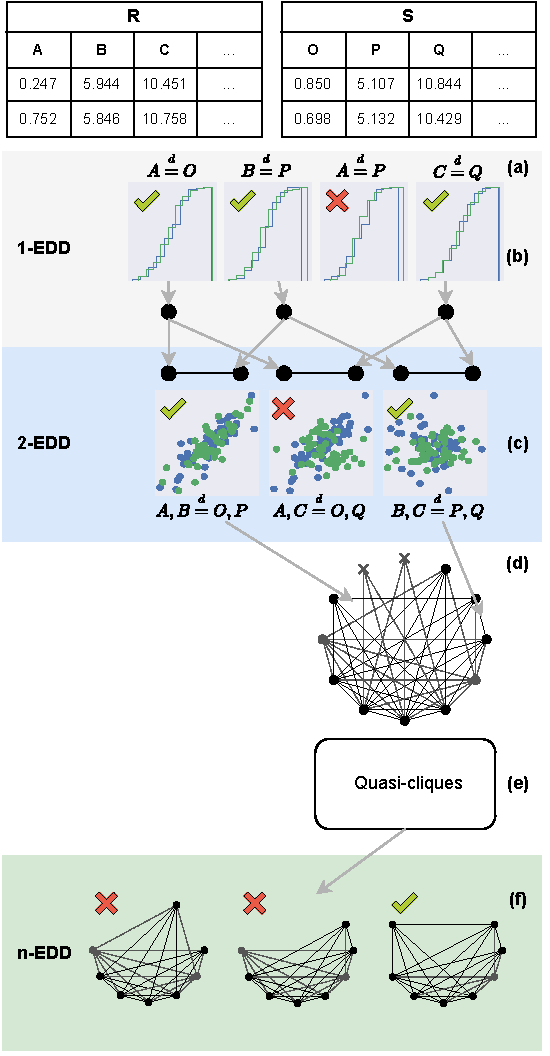
\includegraphics[width=\linewidth]{images/5_presq/pipeline}
    \caption{Simplified schematic of \PresQ.}
    \label{fig:presq_pipeline}
\end{figure}

 Given datasets $R$ and $S$,

(a) Candidate $1$-\glspl{EDD} are found applying the interval-tree as described in section~\ref{sec:presq_unary}.

(b) Those for which the Kolmogorov-Smirnov finds a significant difference are discarded,
    and the rest are mapped to nodes.

(c) All pairwise combinations are tested, and those equally distributed are
    (d) mapped to edges on a 2-hypergraph. The algorithm works with hypergraphs of any rank
    (e.g., triplets mapped to edges on a 3-hypergraph).
    
(e) \PresQ searches for quasi-cliques as described in section~\ref{sec:presq}.

(f) A quasi-clique of cardinality $n$ corresponds to an $n$-EDD, which is then validated by
a statistical test. Those rejected are decomposed to generate the edges for a 3-hypergraph, which are
verified (c), used to build a $3$-hypergraph (d) and finally passed as input back to (e).

The graph above displays spurious nodes and edges (light grey, dotted) and false negatives
(missing edges between dark nodes) based on attribute names. The full graph is not a valid
quasi-clique because the hypergeometric
test on the node degree (eq.~\ref{eq:deg_hyperclique_hypergeom}) prunes the two nodes shown with
crosses.
Three candidates of arity 8 are generated given the constrain on the number of edges 
(eq.~\ref{eq:edge_hyperclique}). Two of them are rejected by the $n$-dimensional statistical test and used to compute the edges of the $3$-hypergraph.

\end{multicols}
    
\newpage

\subsubsection{Parameters}

Before explaining how to tailor the parameterization of the quasi-clique finding for the purpose
of searching \glspl{EDD}, we need to remind that, given two sets of attributes $R[X]$ and $S[Y]$,
our algorithm builds on the null hypothesis $H_0: P(R[X]) = P(S[Y])$.
In other words, it is based on the \emph{assumption} that any \gls{EDD} candidate is valid.

Let $\alpha$ be the significance level chosen by the user before running the algorithm.
Let $G$ be the initial $k$-uniform hypergraph and let $K$ be a quasi-clique candidate.
Under $H_0$, $K$ represents a $|K|$-ary EDD, and by the projection rule,
all possible edges between the nodes in $K$ are also valid $k$-ary \glspl{EDD}.
If we run null hypothesis tests over these $k$-ary specialized \glspl{EDD},
by the definition of type-I error, we can expect as many as $\alpha \times \binom{|K|}{k}$ false rejections.
In other words, under $H_0$, we can expect a ratio of $\alpha$ missing edges.
This is equivalent to setting the threshold for equation~\ref{eq:edge_hyperclique} as:

\begin{equation*}
    \gamma = 1 - \alpha   
\end{equation*}

Adjusting $\lambda$ is less straightforward: a high threshold
will reject good candidates. A low one will accept spurious ones, triggering
unnecessary tests. Even worse, the spurious quasi-cliques tend to have a high cardinality.
Once rejected, they will cascade and cause an increase in lower-arity \glspl{EDD}
to be tested as much as $\binom{n}{k+1}$, where $n$ is the arity of the \gls{EDD} candidate,
and $k$ is the current level of the bottom-up exploration.

To solve this dilemma, we propose to use an adaptive value for $\lambda$ based on the
quasi-clique being checked: under $H_0$, there is no reason to think that any
particular subset of the edges from the clique has a higher probability of
having missing members. In other words, if a given node has an
unexpected low degree, it is most likely connected by spurious edges.

Let $N$ be the number of edges and $n$ the
maximum degree of the nodes on a clique with $|V'|$ nodes. Under this null hypothesis,
the degree of the nodes should roughly follow a hypergeometric distribution:
\begin{equation}
    \Pr(\operatorname{Degree}(v) = d)  = \frac{\binom{|E'|}{d} \binom{N - |E'|}{n - d}}{\binom{N}{n}}, \textrm{ for } v \in V'
    \label{eq:hypergeometric}
\end{equation}
This fact allows us to perform a statistical test and accept or reject our
quasi-clique candidate with a given significance level.
Figure~\ref{fig:hypergeom_sf} shows some examples of this distribution for a
quasi-clique with 29 nodes and the critical value for
a one-tail test with $\alpha = 0.05$. In other words, if the degree of a
node within a quasi-clique candidate is less than the critical value, we can reject the
null hypothesis and accept that the set of edges connecting the node are spurious.

\begin{figure}[ht]
    \centering
    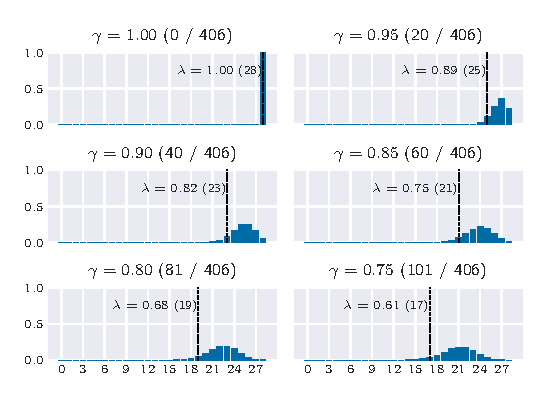
\includegraphics{images/5_presq/hypergeom}
    \caption[Distribution of the degree of the nodes under the assumption that missing edges
    are due to the expected false negative rate.]{
    Distribution of the degree of the nodes under the null hypothesis that the 
    missing edges on the quasi-clique are due to the expected false negative rate of the
    statistical test.
    The vertical line corresponds to the one-tail test with $\alpha = 0.05$.}
    \label{fig:hypergeom_sf}
\end{figure}

In summary, as a constant number of missing edges could be considered
too restrictive \cite{brunato2007effectively}, we consider a fixed ratio to be
limiting as well, and harder to make sense of ---i.e., why choose $\lambda = 0.6$
and not $\lambda = 0.7$?.
We propose that instead, replacing equation~\ref{eq:deg_hyperclique}
with equation~\ref{eq:deg_hyperclique_hypergeom} could be a more intuitive and
flexible approach.
\begin{equation}
    \forall v \in V': \operatorname{CDF}(\operatorname{Degree}(v)) \ge \Lambda
    \label{eq:deg_hyperclique_hypergeom}
\end{equation}
Where $0 \le \Lambda \le 1$. As with $\gamma$ and $\lambda$, a value of 1 would only accept
regular cliques.

The proposed parameterization for $\gamma$ and $\Lambda$ are internally consistent
since they are both constructed under $H_0$.

Figure~\ref{fig:presq_pipeline} visually summarizes the stages of \PresQ algorithm,
and the effects of the parameters $\gamma$ and $\Lambda$ on the quasi-clique finding stage.

In the following section, we will show that adapting \Find clique validation with ours
is enough to improve its performance in run-time and results. The \emph{growing}
step improves the efficacy (i.e. more maximal \glspl{EDD} found) at the cost of a higher run-time.

\section{Experiments}
\label{sec:presq_experiments}
We have implemented in Python a version of \Find that validates candidates with statistical
tests, and the proposed \PresQ.
Both share most of the code, including initialization and statistical
tests. Any difference in run-time is only because the modified version
searches for quasi-cliques instead of full cliques.

We focus on comparing these algorithms for two main reasons:
1) To prove that quasi-clique finding can outperform clique finding both in run-time and
results when the data is noisy, an advantage not necessarily exclusive to \gls{EDD} finding;
2) While \glspl{IND} are targeted towards inferring foreign-key relationships and generally of low arity,
we expect \glspl{EDD} to be of high arity ---\emph{co-located within a multidimensional space}---,
and \Find performs well when the arity is high~\cite{Dursch2019}.

\subsection{Experimental design}
\label{sec:experiment_design}
We have performed two different sets of experiments: one exclusively benchmarks the
quasi-clique search, while the other runs over real-world datasets.

\subsubsection{(Quasi-) clique search}
This experiment decouples the testing of the quasi-clique search from the uncertainty
associated with the data. The test accepts as parameters the rank
for the hyper-graph $k$, the cardinality for the clique $n$, the number of additional
nodes $N$, the fraction of missing edges $\alpha$ and the fraction of \emph{spurious}
edges $\beta$.
With these parameters, the test performs the following initialization procedure:

\begin{enumerate}
    \item Create $n$ nodes belonging to the clique
    \item Create $N$ additional nodes
    \item Create the set $E$ of $\binom{n + N}{k}$ edges connecting \emph{all nodes}
    \item Create the set $Q$ of $\binom{n}{k}$ edges belonging to the clique
    \item Obtain the set of all edges not belonging to the clique $C = E \setminus Q$
\end{enumerate}

With these sets, and to obtain an estimation of the distribution of the target measurement,
it then repeatedly generates noisy versions of the original clique through the following steps:

\begin{enumerate}
    \setcounter{enumi}{5}
    \item Remove $\alpha \times |Q|$ random edges from the original full clique $Q$
    \item Add $\beta \times |C|$ random edges from $C$
    \item Run \Find and \PresQ over the resulting graph
\end{enumerate}

The parameters $\alpha$ and $\beta$ simulate the effect of type I and type II errors
respectively.

\PresQ is configured with $\gamma = 1 - \alpha$ and $\Lambda = 0.05$. The number of additional nodes
is fixed to half the number of nodes in the clique: $N = \frac{n}{2}$.

This experiment measures, in a controlled manner, the capability of the
algorithms to find the \emph{true} clique and how their run-time is affected by the number of
missing and spurious edges.
Since the inputs are randomized, some will unavoidably run with exponential complexity,
the worst case for all the algorithms. To avoid spending too much time on these extreme cases,
the test also accepts a timeout parameter.
We describe the measurements we have taken in table \ref{tab:quasi_measurements}, and
the different parametrizations in table \ref{tab:quasi_params}.

\begin{table}[tbp]
    \caption{Set of measurements taken for the quasi-clique finding problem.}
    \label{tab:quasi_measurements}
    \centering
    \begin{tabular}{p{0.23\linewidth} p{0.7\linewidth}}
        \emph{Recovery ratio} & For each quasi-clique $Q'$ found, we compute the
        Jaccard index for each found quasi-clique,
        $J(Q, Q') = {|Q \cap Q'| \div |Q \cup Q'|}$.
        From all the obtained values, we report the maximum. A value of
        $1$ signals a perfect match. \\
        \emph{Time}           & Wall-clock time. \\
        \emph{Timeouts}       & How many runs exceeded the timeout. \\
    \end{tabular}
\end{table}

\begin{table}[tbp]
    \caption{Combination of parameters for the quasi-clique find problem.}
    \label{tab:quasi_params}
    \centering
    \begin{tabular}{c c c c r}
    \thead{Rank} & \thead{$\alpha$} & \thead{$\beta$} & \thead{Timeout (s)} \\
    \multirow{2}{*}{$2$} & $[0.05, 0.30]$, step $0.05$ & $0.0$ & \multirow{2}{*}{$240$} \\
    & $0.1$ & $[0.0 - 0.8]$ step 0.2 & \\[0.5cm]
    
    \multirow{2}{*}{$3$} & $[0.05, 0.30]$, step $0.05$ & $0.0$ & $300$ \\
    & $0.1$ & $[0.0 - 0.8]$ step 0.2 & $1200$ \\[0.5cm]
    
    \multirow{2}{*}{$4$} & $[0.05, 0.30]$, step $0.05$ & $0.0$ & $1200$ \\
    & $0.1$ & $[0.0 - 0.8]$ step 0.2 & $3000$ \\
    \end{tabular}
\end{table}

\subsubsection{Real-world datasets}
For the statistical tests, we use a non-parametric multivariate test based on
\gls{kNN}~\cite{Henze1988,Schilling1986b}, but any other multivariate
test could be used. However, regardless of the chosen test, there will always
be a number of false negatives bound by the significance level. In any case, the techniques
here discussed remain relevant.

The initialization stage of the test is as follows:

\begin{enumerate}
    \item We load two separate datasets.
    \item The constant columns, where every tuple has the same value ---including \emph{null}---
        or only a handful of different values, are dropped. \textsc{Faida} authors followed
        a similar procedure to reduce the number of columns to check \cite{Kruse2017}.
    \item A random sample is taken from both relations (it defaults to 200).
    \item The algorithm described in section~\ref{sec:presq_unary} is used to find a set of valid
        unary \glspl{EDD}.
    \item \emph{All} possible $n$-EDDs (for $n \in \{2, 3\}$) are generated and validated.
        The tests begin at different arities in order to compare the resiliency of
        \Find and \PresQ for different initial conditions.
    \item Valid $n$-EDDs are used to create the initial graph passed as input to \PresQ.
\end{enumerate}

The fifth step is performed at different significance levels of
$\alpha \in \{0.05, 0.10, 0.15\}$
to verify how the number of missing and spurious edges affects the search algorithms.
Typically, \Mind would generate the graph (i.e. 3-EDDs are generated from valid 2-EDDs).
Nonetheless, we start with all possible $n$-EDDs for simplicity: it is easier to
model and understand how many missing edges are expected as a function of $\alpha$.

The input for both search algorithms is, thus, identical at every run. However, since
there is an unavoidable effect of the randomization of the sampling in step 3 and the
$N$-dimensional permutation tests, we repeated the experiment.
As a result, we are confident that the difference is significant and not due to chance.

While \Find has no parameters beyond the initial set of \glspl{EDD},
\PresQ requires a value for both $\gamma$ and $\Lambda$. As we mentioned earlier,
it makes sense to bind $\gamma$ to the expected number of missing edges
(false negatives): $\gamma = 1 - \alpha$. For $\Lambda$, we tested with the
values 0.05 and 0.1 since lower values yield too many accidental quasi-cliques,
while higher values defeat the tolerance introduced by $\gamma$.

To measure the efficacy (\glspl{EDD} finding) and efficiency (run-time) of the algorithms,
we took the measurements summarized in tables \ref{tab:raw_measurements}
and \ref{tab:derived_measurements}.

\begin{table}[tbp]
    \caption{Set of measurements taken from individual runs.}
    \label{tab:raw_measurements}
    \centering
    \begin{tabular}{p{0.28\linewidth} p{0.63\linewidth}}
        \emph{Time}  & Wall-clock time, without accounting for the initialization stage,
                       as this is shared. \\
        \emph{Number of tests} & Time spent looking for quasi-cliques and validating the
                                   candidates.
                                   Tests can be potentially expensive, so we measure how many
                                   statistical tests are necessary. \\
        \emph{EDD count} & Without removing non-maximal \glspl{EDD}. \\
        \emph{Maximal EDD count} & Removing non-maximal \glspl{EDD}. \\
        \emph{Timeouts} & The execution time has a time limit of 3000 seconds. We report the
         percentage of runs that could not finish within the allocated time window. \\
        \emph{Highest arity} & The maximum \gls{EDD} arity found. \\
    \end{tabular}
\end{table}

\begin{table}[ht]
    \caption{Set of measurements derived over the complete set of runs.}
    \label{tab:derived_measurements}
    \centering
    \begin{tabular}{p{0.16\linewidth} p{0.75\linewidth}}
        \emph{Match ratio} & It is a ratio between the maximum arity of the maximal
        quasi-clique found and the \textit{true} maximum \gls{EDD} possible to find on
        each separate run.
        This \emph{truth} is solely based on attribute names. The algorithms can
        find higher arity \glspl{EDD} when the values are taken into account.
        This is proof of success: the metadata would not have sufficed to capture
        this trait. \\
        
        \emph{Accuracy} & Measured as the number of total returned \glspl{EDD}, divided by
        the number of statistical tests executed. A ratio of $1$ (best) means that every
        candidate was accepted by the statistical test, while a ratio of $0$ (worst)
        means that all candidate quasi-cliques were rejected. This value is
        also affected by the power of the statistical test as a function of
        dimensionality.\\
    \end{tabular}
\end{table}

Given the variability and the number of dimensions, it can be hard to assess the quality
of the results. As a general guideline, we consider:

\begin{itemize}
    \item The higher the match ratio, the better: the highest arity EDD
    is potentially the most interesting and selective candidate for cross-matching.
    \item For a similar match ratio, the lower the run-time, the better.
\end{itemize}

For a similar match ratio, a higher number of maximal \glspl{EDD} is desirable. Arguably not
for the \gls{IND} discovery ---after all, a few good candidates may suffice---,
but it proves the capacity of finding maximal quasi-cliques.

It is important to note that some of these measures are interdependent. For instance,
if a maximal \gls{EDD} with a higher arity is found, the number of \glspl{EDD} should generally decrease.
Conversely, if a true, high-arity candidate is rejected, multiple generalizations will be considered
and possibly accepted, increasing the number of unique \glspl{EDD}.
Similarly, finding more maximal \glspl{EDD} implies running more statistical
tests, so the run-time will be worse. Ultimately, it is up to the user to decide what is
more important and parameterize the algorithm accordingly.

We ran the tests disabling the limitation on the degree ($\Lambda = 0$) and
the limitation on the total number of edges ($\gamma = 0$). In this manner, we can
evaluate if there is any difference when using one, the other, or both.

\begin{table}[ht]
    \caption{Summary of the datasets used for validation.}
    \label{tab:dataset_summary}
    \centering
    \begin{tabular}{l c r r r}
        \textbf{Dataset}   & \textbf{Tables} & \textbf{Rows} & \textbf{Columns} & \textbf{1-EDD} \\
        Mortgage/Treasury  & 2               &   1k + 1k   & 16 + 16 &  26 \\
        Ailerons/Elevators & 2               &  14k + 17k  & 41 + 19 &  44  \\
        DC2                & 2               & 198k + 193k & 39 + 33 & 279 \\
        AFDS               & 4               & $172 \times 4$ & $8 \times 4$ & 63 \\
        Waveform           & 2               & 5k + 5k     & 22 + 41 & 145 \\
        KEEL      & 43              & 43 --- 41k  & 444 & 972 \\
        ChEMBLDB           & 79              & 5 --- 19M   & 418 & 599 \\
    \end{tabular}
\end{table}

\textbf{Datasets:} To test the algorithms, we ran them over two pairs of relations from the KEEL
regression datasets \cite{alcala2011keel}, the training and test catalog from the
\textit{Euclid photometric-redshift challenge} \cite{EuclidDesprez2020},
and a set of sensor measurements from an aircraft fuel distribution
system \cite{Gheraibia2019}. For the scalability tests, we have used the full
KEEL regression dataset, two variants from the Waveform Database
Generator~\cite{Dua:2019,breiman_classification_1984},
and versions 29 and 30 of the ChEMBL database~\cite{gaulton_chembl_2016}.

Some statistics about these datasets are summarized in table~\ref{tab:dataset_summary}.

\emph{Mortgage / Treasury}, from KEEL, contain the same data, permuted by rows and by 
columns. These datasets are an example of data de-duplication.

\emph{Ailerons / Elevators}, also from KEEL, share their origin (control of an F16 
aircraft) but have different sets of attributes. These datasets are an example of 
data fusion.

\emph{DC2} comes from a single catalog of astronomical
    objects split based on the sky coordinates.
    The authors masked some of the attributes of the training set (i.e., coordinates and the
    target attributes red-shift). 
    Therefore, both catalogs share some of the attributes but from different sources.
    A naive one-to-one schema matching will
    easily mistake these attributes for small sample sizes. In contrast, for bigger samples,
    some true correspondences will be falsely rejected.
    These datasets require some more resilient methods capable of working on a
    multidimensional space.
    These datasets are an example of schema inference/matching and automatic feature discovery.
    
\emph{\gls{AFDS}} comprises five different files,
    all sharing the same schema but containing sensor measurement values for different scenarios:
    one nominal, and four abnormal. Our implementations of \Find and \PresQ can process
    the five files at the same time.

\emph{Waveform Database Generator}
    We use version 1, with 21 attributes, and version 2, which shares the same 21 attributes and adds 19
    extra features that are just Gaussian noise. This 21-ary \gls{EDD} between the datasets goes
    beyond the maximum 7-ary evaluated in previous works~\cite{Dursch2019}.
    Additionally, the number of attributes and their distribution similarity generates many false positives at low
    dimensionality, stressing the capability of processing noisy, dense, graphs.

\emph{ChEMBL Database}
    We use versions 29 and 30 of the ChEMBL database, each of size 20GiB. They are
    stored on \textsc{BeeGFS}, a clustered filesystem. We evaluate the scalability with respect to the number of
    columns, adding tables progressively. In this scenario, the overhead introduced by the sampling becomes significant.

The two pairs from KEEL (i.e. Mortgage/Treasury and Ailerons/Elevators) were found
running over the whole KEEL dataset initial versions of the algorithms described in
this paper, proving their capabilities. We report the performance of this exercise, together
with the other two scalability tests, in section \ref{sec:scalability}.

\subsection{Environment}

The tests were run on a cluster, where each node
is fitted with an Intel(R) Xeon(R) Gold 6240 CPU at 2.60GHz with 36 virtual cores,
running on a standard CentOS Linux 7.9. The default memory allocation per core was
3 GB. 

For the (quasi-)clique search, we submitted one job with as many tasks as
parameter combinations described in table \ref{tab:quasi_params} and 1 CPU per task,
for cliques of size $10, 20$, and $30$.  We chose the time limit based on the measured
run-time from early test runs.

For the real dataset tests, we submitted jobs with 8 tasks and 1 CPU per task,
limited to 24 hours. The objective of concurrent runs was to increase the number
of data points since the code was not parallelized.

Finally, we executed ten randomized runs for each increment on the number of columns for the scalability tests.

\subsection{Results}
\label{sec:results}

In this section, we summarize the results of our test setup.

\subsubsection{(Quasi-) clique search}
\label{sec:result_quasi_search}

We summarize the \emph{wall-time} and \emph{recovery ratio} metrics by estimating
their distribution mean and its associated standard error following the Bootstrap method.
The \emph{timeout} is measured by counting how many runs fail to find a quasi-clique within
the allocated time window.

While the \emph{wall-time} distribution is far from Gaussian, we consider that randomizing the
input, pruning the long-running cases, and averaging the results of a few
short-running iterations is a valid usage of the algorithms.
This makes comparing the means a reasonable assessment.

\textbf{Influence of spurious edges:}
We show in figure~\ref{fig:3hyper_beta} the performance of the algorithms for $3$-hypergraphs
and different ratios of spurious edges. The exponential worst-case
complexity becomes more apparent the more connected nodes there are.
\Find is the most affected, but at some point, \PresQ performance also degrades significantly and eventually also fails to finish on time.
These results confirm that spurious edges influence the
\emph{run-time} of these algorithms very negatively~\cite{koeller2006heuristic}.

\begin{figure}[ht]
    \centering
    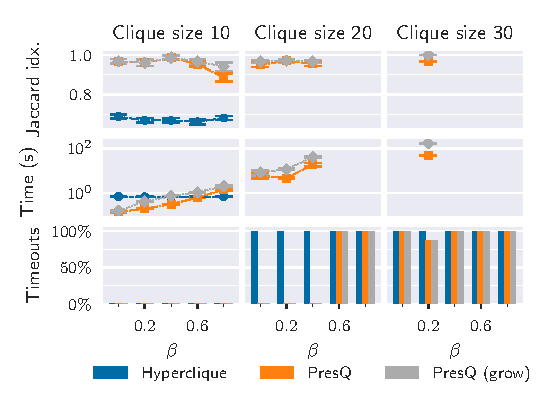
\includegraphics{images/5_presq/3hyper_beta}
    \caption[Recovery ratio and run-times for cliques on uniform $3$-hypergraphs for different ratios of spurious edges.]{
        Recovery ratio and run-times for cliques on uniform $3$-hypergraphs
        for different ratios of spurious edges ($\beta$).
        Each data point corresponds to 15 runs.
    }
    \label{fig:3hyper_beta}
\end{figure}

\textbf{Influence of missing edges:}
Figure~\ref{fig:3hyper_alpha} shows that our proposal
generalizes for hypergraphs. \PresQ with the growing stage enabled, oscillates very close
to the original clique even when $30\%$ of the edges are missing. However, the number of
timeouts increases given that the algorithm needs to traverse more levels from the seed to the maximal
quasi-clique. Interestingly, there is an inverse correlation between the number
of missing edges and run time.

\begin{figure}[ht]
    \centering
    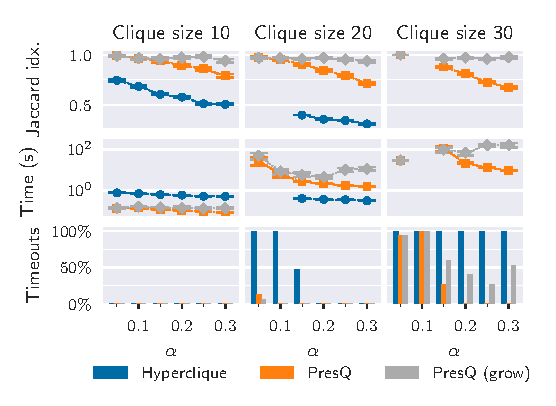
\includegraphics{images/5_presq/3hyper_alpha}
    \caption[Recovery ratio and run-times for cliques on uniform $3$-hypergraphs
    for different ratios of missing edges.]{Recovery ratio and run-times for cliques on uniform $3$-hypergraphs
    for different ratios of missing edges ($\alpha$).
    Each data point corresponds to 15 runs.}
    \label{fig:3hyper_alpha}
\end{figure}

\textbf{Influence of correlated ratios:}
In a more realistic scenario --- i.e., when using statistical tests --- as the number of missing edges
increases, the number of spurious edges should decrease.
We have run tests with the growing stage enabled for different parametrizations on the node degree
threshold. This includes a regular $\lambda$ parameter with a value of $0.8$ chosen based on
good empirical results we obtained during early iterations of this work.
The correlation between $\beta$ and $\alpha$ is based on the empirical statistical power of the
\gls{kNN} test as a location test on $k$ dimensions and a sample size of 100.
In all cases, $\gamma = 1 - \alpha$.

Figure~\ref{fig:hyper_ab_corr} summarizes the results. A hand-picked parameter of $\lambda = 0.8$ can
perform well for some hypergraphs but quickly underperforms as the hypergraphs become noisier.
On the contrary, our proposal based on the hypergeometric distribution remains stable.
However, disabling the degree limitation performs better for this particular setup.
This makes sense since there is no correlation between missing edges.

\begin{figure}[ht]
    \centering
    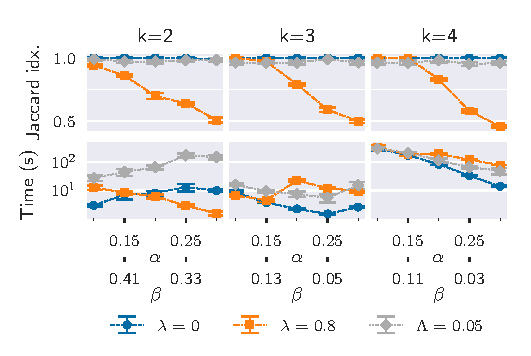
\includegraphics{images/5_presq/quasi_corr_20}
    \caption[Recovery ratio and run-times for cliques of size 20 on uniform $(2,3,4)$-hypergraphs.]{
    Recovery ratio and run-times for cliques of size 20 on uniform $(2,3,4)$-hypergraphs.
    In this setup, there were no timeouts. Each data point corresponds to 5 runs.
    }
    \label{fig:hyper_ab_corr}
\end{figure}

\subsubsection{Real-world datasets}
\label{sec:results_real}

The initial randomized state heavily influences the proposed performance measurements.
Their distribution can not be assumed normal.
Purely comparing their means is not enough to assess the validity of our proposal, and we also need an estimation of variability.

The metric of choice used to compare our measurements is the \emph{percent difference}
between sample means, being its sample estimator~\cite{campelo_sample_2019}:

\begin{equation}
    \label{eq:percent_difference}
    \hat{\phi} = \frac{\hat{\mu}_{\PresQ} - \hat{\mu}_{\Find}}{\hat{\mu}_{\Find}}
\end{equation}

The distribution of
$\hat{\phi}$ can be estimated using bootstrapping.
In this manner, we obtain the estimated population mean and standard deviation. Finally,
we compute the $95\%$ confidence interval $\hat{\mu_\phi} \pm 1.96 \hat{\sigma_\phi}$

Figure~\ref{fig:results_summary} shows this confidence interval for match ratio, unique \glspl{EDD},
number of tests and wall time (columns) for a significance level of $0.10$, against the
different datasets (rows).

\begin{figure}[htbp]
    \centering
    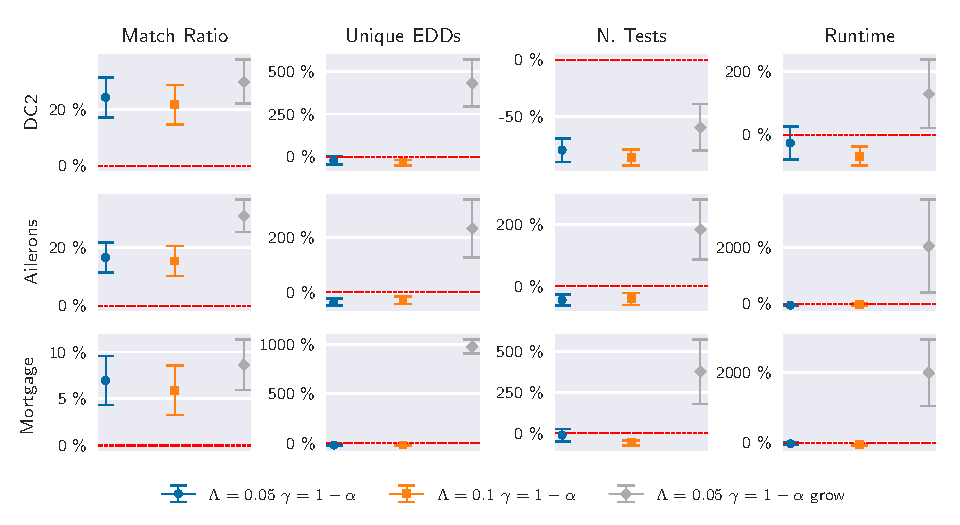
\includegraphics[width=\linewidth]{images/5_presq/all}
    \caption[$95\%$ confidence intervals for the percent difference between \Find and \PresQ.]{
        $95\%$ confidence intervals for the percent difference
        (equation \ref{eq:percent_difference}) between \Find and
        three parameterizations of \PresQ for the DC2, Ailerons vs. Elevator, and
        Mortgage vs. Treasury datasets.
        Intervals that do not intersect the horizontal dashed line at $0\%$  show a statistically
        significant result.
        For ratio, higher is better. For tests and run-time, lower is better. Unique is harder to
        assess since the results also depend on the statistical power of the chosen test.
        Since the growing stage can generate many candidates, a low-powered test will accept
        many false \glspl{EDD}.
    }
    \label{fig:results_summary}
\end{figure}

The DC2 case is particularly interesting. The attributes of the datasets
are relatively numerous ---compared to the others--- and very similar in their distributions.
A low initial significance level will generate very dense graphs, with a few missing edges, and
many spurious, which impacts the performance considerably.
This is a known issue of \Find~\cite{koeller2006heuristic}.
Increasing the significance level reduces the number of spurious edges at the cost of
missing true ones. Consequently, the efficiency is improved at the cost of the efficacy.
\PresQ allows us to increase the significance
level without sacrificing much efficacy.

For the \gls{AFDS} dataset, when comparing the maximum \gls{EDD} arity found per pair of files,
scenarios two and three are the most similar, as seen in figure~\ref{fig:afds}.
We can obtain this insight without even knowing what the schema nor the content of the files are.
After seeing this result, we checked the original paper from
where the dataset was obtained, verifying that, indeed, they are
``two closely related scenarios'' \cite{Gheraibia2019}.
We consider this another proof of the utility of the proposed techniques.


\begin{figure}[ht]
    \centering
    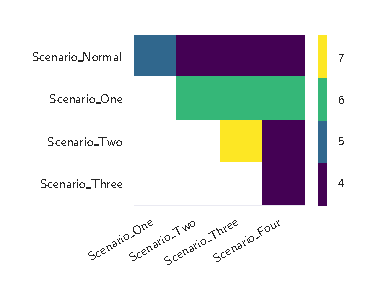
\includegraphics[width=0.5\linewidth]{images/5_presq/afds}
    \caption{
        Pairwise max arity found on the \glsfmtshort{AFDS} dataset for each pair of scenarios.
    }
    \label{fig:afds}
\end{figure}

Table~\ref{tab:ind2_summary} (page \pageref{tab:ind2_summary}) summarizes
the overall results when
we execute our tests over the datasets \emph{Mortage vs Treasury},
\emph{Ailerons vs Elevators} and \emph{DC2} for different values of $\gamma$ and $\Lambda$ ---
note that \Find is equivalent to either of the two parameters set to $1.0$. For run-time,
match ratio, and the number of unique \glspl{EDD}, we provide the first and third quartiles.
The \emph{precision} column shows how many candidates are accepted by the
statistical test. A value of $1$ means that all candidates were valid \glspl{EDD}.

When the search algorithm looks for cliques (the first entry for each dataset),
the precision is high since almost all candidates were accepted. However,
these candidates are, on average, of lower arity. This is visible on the \emph{Match}
columns. As the potential maximal arity becomes higher ---e.g., \emph{DC2}--- the
chance of having missing edges increases, thus making the search more resource intensive.

On the other hand, in a too-permissive setup where only $\gamma$ constrains the quasi-cliques
(second entry), the algorithm is too eager and accepts \gls{EDD} candidates later rejected either
by the statistical test or by the limitation of not accepting duplicated columns.
The precision is low, and the search time increases as well.

Our proposed $\Lambda$ parameter, based on the \emph{expectation} on the number of missing edges,
is more effective at constraining the set of candidates even when used alone (third entry).
The precision increases and the run time is reduced.
When combined with $\gamma$ (fourth and fifth entries), the precision increases
and fewer tests are required.

As an illustration of this balance, let us examine in more detail the consequences of the
different $\Lambda$ parameterization following the process shown in figure~\ref{fig:presq_pipeline}
when running over the DC2 dataset. The first four stages are unaffected by this parameter:

\begin{enumerate}[label=({\alph*}),align=parleft,leftmargin=!,labelwidth=1em]
\item As described in section~\ref{sec:presq_unary}, an interval tree is built over the attributes
    from both relations. Only overlapping ranges are compared,
    reducing by $~27\%$ the number of tests required.
\item $~810$ KS tests need to be done. $~49$ pairwise combinations are considered equally distributed
    (\glspl{uEDD}).
\item $(n \times (n - 1)) \div 2 ~= 1176$ edges are build combining all \glspl{uEDD} and validated
    using the \gls{kNN} test. $~612$ edges are considered valid.
\item The initial graph has half as many edges as the complete graph.
    Since we know the ground truth, we can extract the sub-graph induced by the set of
    true \gls{uEDD} and find the number of missing edges to be $\approx 0.10$ on average,
    as we expected.
\end{enumerate}

\medskip

The following table exemplifies the consequences of different values of $\Lambda$
--- see equation~\ref{eq:deg_hyperclique_hypergeom} --- on
the count and size of the found quasi-cliques (e) and the number validated by the \gls{kNN} test (f).
Those invalid are `decomposed' into candidate $3$-EDDs, validated, and 
used to build a $3$-hypergraph (d) feedback to stage (e) for the next iteration.

\begin{center}
\begin{tabular}{lrrr}
                   & \thead{Quasicliques} & \thead{Valid} & \thead{Median size} \\
$\Lambda = 0.00$   & 2385                 & 292       & 19        \\
$\Lambda = 0.05$   & 107                  & 64        & 12        \\
$\Lambda = 1.00$\footnotemark & \numprint{53 053} & \numprint{52 291} &  6         \\
\end{tabular}
\end{center}

\footnotetext{Equivalent to clique finding}

\medskip

For $\Lambda = 0$, the search algorithm is too greedy and accepts quasi-cliques that are poor candidates.
Too many are invalid and need to be feedback to the algorithm, increasing run-time.
For $\Lambda = 1$, the search algorithm is too restrictive. Its precision is high,
but it spends a long time enumerating small cliques. $\Lambda = 0.05$ provides
the right balance, improving the result and performance.

Finally, the growing stage increases the number of candidates of all arities.
This requires a more exhaustive traversal of the search space and the execution of more tests,
increasing the total run-time. While we run the growing stage over
\emph{all} found seeds, this stage could be restricted only
to a subset of the most interesting \emph{seeds} ---e.g., highest cardinality.

% Results starting arity 2
\begin{table}[htbp]
    \caption[Summary of run-time, matching ratio, and number of maximal quasi-cliques found.]{
        Summary of run-time, matching ratio (based on name), and number of maximal quasi-cliques found
        accepted by the statistical test.
        The significance level is $\alpha = 0.1$.
        $N$ corresponds to the number of randomized runs.
        \PresQG identifies \PresQ with the growing stage.
    }
    \label{tab:ind2_summary}
    \centering
    \resizebox{\textwidth}{!}{%
    \begin{tabular}{l r r | r r | r r | r r | r | r | r}
    
    \multicolumn{11}{c}{\textit{Mortgage vs Treasury}} \\
    
    & \thead{$\Lambda$} & \thead{$\gamma$} & \multicolumn{2}{c|}{\thead{Time (s)}} &
        \multicolumn{2}{c|}{\thead{Match}} & \multicolumn{2}{c|}{\thead{Unique}} &
        {\thead{Prec.}} & {\thead{N}} & \thead{Timeouts} \\

    & & & \textit{Q1} & \textit{Q3} & \textit{Q1} & \textit{Q3} & \textit{Q1} & \textit{Q3} & \\ \hline
    
    \Find   &                &               &   0.44 &   0.64 & 0.75 &	1.00 &  12 &  21 & 0.99 & 527 & 0.0\% \\
    \PresQ  & \bfseries 0.00 &           0.9 &  44.86 & 459.04 & 0.94 & 1.00 &  11 &  15 & 0.06 & 212 & 0.0\% \\
    \PresQ  &           0.05 & \bfseries 0.0 &   0.71 &  11.08 & 0.88 & 1.00 &  11 &  17 & 0.49 & 535 & 0.0\% \\
    \PresQ  &           0.05 &           0.9 &   0.76 &  10.61 & 0.88 &	1.00 &  11 &  17 & 0.57 & 507 & 0.0\% \\
    \PresQ  &           0.10 &           0.9 &   0.73 &   1.99 & 0.84 & 1.00 &  11 &  17 & 0.75 & 503 & 0.0\% \\
    \PresQG &           0.05 &           0.9 &  47.10 &	247.39 & 0.88 &	1.00 & 125 & 262 & 0.22 & 503 & 0.0\%\\

    \\
    \multicolumn{11}{c}{\textit{Ailerons vs Elevators}} \\
    
    \Find   &                &               &  5.63 &  48.41 & 0.78 & 1.00 & 142 &	 291 & 0.98 &  93 & 0.0\% \\
    \PresQ  & \bfseries 0.00 &           0.9 &  8.82 &  36.75 & 1.00 & 1.22 &  88 &  174 & 0.24 & 128 & 0.0\% \\
    \PresQ  &           0.05 & \bfseries 0.0 & 22.68 &  52.87 & 1.00 & 1.22 & 113 &  239 & 0.16 & 126 & 0.0\% \\
    \PresQ  &           0.05 &           0.9 &  7.51 & 	20.12 &	1.00 & 1.11 &  86 &	 198 & 0.35 &  60 & 0.0\% \\
    \PresQ  &           0.10 &           0.9 &  6.83 & 	22.40 & 1.00 & 1.11 &  89 &	 205 & 0.41 &  60 & 0.0\% \\
    \PresQG &           0.05 &           0.9 & 57.86 & 674.26 &	1.11 & 1.25 & 321 &	1062 & 0.22 &  60 & 0.0\% \\
    
    \\
    \multicolumn{11}{c}{\textit{DC2}} \\
    
    \Find   &                &               &   74.94 &  805.71 & 0.60 & 0.71 &  73 & 150 & 0.90 &  53 & 34.0\% \\
    \PresQ  & \bfseries 0.00 &           0.9 &  681.51 & 1536.19 & 0.68 & 0.69 & 102 & 200 & 0.01 &  16 & 87.5\% \\
    \PresQ  &           0.05 & \bfseries 0.0 &  40.07 &   189.45 & 0.80 & 0.93 &  46 & 115 & 0.10 &  21 & 47.6\% \\
    \PresQ  &           0.05 &           0.9 &   25.57 &  214.27 & 0.76 & 0.89 &  46 & 113 & 0.14 &  53 & 13.2\% \\
    \PresQ  &           0.10 &           0.9 &   18.61 &  144.98 & 0.76 & 0.87 &  42 &  98 & 0.18 &  52 & 23.1\% \\
    \PresQG &           0.05 &           0.9 &  458.26 & 1881.02 & 0.81 & 0.93 & 518 & 798 & 0.23 &  52 & 50.0\% \\
    \end{tabular}}
\end{table}

% Results starting at arity 3
\begin{table}[htpb]
    \caption[Summary of run-time, matching ratio, and number of maximal quasi-cliques found with an initial arity $k = 3$.]{
        Summary of run-time, matching ratio (based on name), and number of maximal quasi-cliques found.
        Significance level is $\alpha = 0.1$, initial arity $k = 3$.
    }
    \label{tab:ind3_summary}
    \centering
    \small
    \resizebox{\textwidth}{!}{%
    \begin{tabular}{l r r | r r | r r | r r | r | r | r}
    
    \multicolumn{11}{c}{\textit{Mortgage vs Treasury}} \\
    
    & \thead{$\Lambda$} & \thead{$\gamma$} & \multicolumn{2}{c|}{\thead{Time (s)}} &
        \multicolumn{2}{c|}{\thead{Match}} & \multicolumn{2}{c|}{\thead{Unique}} &
        {\thead{Prec.}} & {\thead{N}} & \thead{Timeouts} \\
        
    & & & \textit{Q1} & \textit{Q3} & \textit{Q1} & \textit{Q3} & \textit{Q1} & \textit{Q3} & & \\ \hline
        
    \Find    &                &             &   8.75 &  20.54 & 0.75 & 1.00 &  86 & 144 & 1.00 & 160 & 16.3\% \\
    \PresQ   &  \textbf{0.00} &         0.9 &  55.00 & 569.01 & 1.00 & 1.00 &  67 & 102 & 0.17 & 160 &  0.0\% \\
    \PresQ   &           0.05 &         0.9 &   8.43 &  19.45 & 0.81 & 1.00 &  82 & 126 & 0.99 & 160 &  0.0\% \\
    \PresQ   &           0.10 &         0.9 &   9.04 &  19.60 & 0.81 & 1.00 &  83 & 130 & 0.99 & 160 &  0.0\% \\
    \PresQG  &  \textbf{0.00} &         0.9 &   6.71 & 902.57 & 0.87 & 1.00 &  98 & 264 & 0.29 & 160 & 47.5\% \\
    \PresQG  &           0.05 &         0.9 &  36.83 & 358.53 & 0.86 & 1.00 & 204 & 395 & 0.98 & 160 &  0.6\% \\
    \PresQG  &           0.10 &         0.9 &  43.23 & 287.59 & 0.81 & 1.00 & 198 & 376 & 0.98 & 160 &  0.0\% \\
        
    \\
    \multicolumn{11}{c}{\textit{Ailerons vs Elevators}} \\
    
    \Find    &                &               &  24.66 & 1072.74 & 0.89 & 1.00 & 474 &  947 & 1.00 & 114 & 40.4\% \\
    \PresQ   &   \textbf{0.00}&           0.9 &  28.55 &  140.93 & 1.13 & 1.33 & 276 &  627 & 0.45 & 114 &  1.8\% \\
    \PresQ   &           0.05 &           0.9 &  26.59 &   83.72 & 1.11 & 1.22 & 339 &  656 & 0.95 & 114 & 14.0\% \\
    \PresQ   &           0.10 &           0.9 &  25.55 &  105.93 & 1.00 & 1.14 & 357 &  680 & 0.96 & 110 & 14.6\% \\
    \PresQG  &  \textbf{0.00} &           0.9 & 171.81 &  940.15 & 1.19 & 1.33 & 498 & 1044 & 0.34 & 114 &  9.7\% \\
    \PresQG  &           0.05 &           0.9 & 174.88 &  670.84 & 1.13 & 1.29 & 629 & 1330 & 0.95 & 111 & 18.9\% \\
    \PresQG  &           0.10 &           0.9 & 205.63 &  718.51 & 1.12 & 1.29 & 661 & 1245 & 0.95 & 109 & 19.3\% \\

    \\
    \multicolumn{11}{c}{\textit{DC2}} \\
    
    \Find    &                &               & 1050.56 & 1050.56 & 1.00 & 1.00 & 560 & 560 & 0.97 & 83 &  98.8\% \\
    \PresQ   &  \textbf{0.00} &           0.9 &  599.20 &  599.20 & 0.88 & 0.88 & 830 & 830 & 0.06 & 32 &  96.9\% \\
    \PresQ   &           0.05 &           0.9 &  207.28 & 2013.45 & 0.81 & 0.89 & 351 & 747 & 0.56 & 81 &  88.9\% \\
    \PresQ   &           0.10 &           0.9 &   71.85 &  926.94 & 0.80 & 0.93 & 380 & 791 & 0.72 & 78 &  93.6\% \\
    \PresQG  &  \textbf{0.00} &           0.9 &         &         &      &      &     &     &      & 32 & 100.0\% \\
    \PresQG  &           0.05 &           0.9 &  340.72 &  599.10 & 1.02 & 1.21 & 775 & 888 & 1.00 & 80 &  97.5\% \\
    \PresQG  &           0.10 &           0.9 &  413.58 &  670.53 & 1.00 & 1.13 & 808 & 947 & 1.00 & 76 &  97.4\% \\
    \end{tabular}}
\end{table}

Table~\ref{tab:ind3_summary} (page \pageref{tab:ind3_summary})
summarizes the performance measures when \Find and \PresQ are run over an initial
3-hypergraph. The precision is considerably higher than when starting on a 2-hypergraph.
This is due to the higher power of the statistical test at dimension 3, so fewer spurious edges are introduced.
However, the overall run-time suffers because the number of edges on a hypergraph is $\binom{|V|}{k}$ where $|V|$ is the number of nodes and $k$ the rank of the hypergraph.
Therefore, for a fixed number of nodes, the number of edges is generally higher for hypergraphs of higher rank.

\subsubsection{Scalability tests}
\label{sec:scalability}

For measuring the scalability of our algorithm, we executed the algorithm over the KEEL, Waveform, and ChEMBL datasets, progressively adding columns, measuring run-time; the
number of $1$, $2$, and $n$-EDDs; and the number of unary tests saved by the interval
tree.
In all cases the chosen parameterization is $\alpha=0.1$, $\Lambda = 0.05$,
$\gamma = 1 - \alpha$ and 200 samples. We set the run-time limit at 3000 seconds.
The relations and their attributes are consistently added in alphanumeric order.
The accepted $1$-EDDs are used to compute all the possible $2$-EDDs, while the accepted $2$-EDDs
define the initial edges for the $n$-EDD finding.
Figure~\ref{fig:scalability} (page~\pageref{fig:scalability}) summarizes our results.


The \emph{KEEL} dataset contains 43 different relations. The interval tree saves around 45\% of
the tests since many columns do not overlap. The number of \glspl{EDD} increments in `bursts' when a
relation that matches a previous one enters the pool. This is due to the existence of
high arity \glspl{EDD} (16, 12, 7, and 6).
The high number of $2$-EDDs makes the growing stage eventually impractical.

For the \emph{ChEMBL} databases, we have used a naive random sampling that only requires a single
pass over the entire database. Even then, the reading time is little with respect to the rest of the EDD
finding algorithm. The number of $1$-EDDs steadily increments as relations are added, but $2$
and $n$-EDDs remain relatively stable ---the corresponding error bars overlap---, and so does the run-time.
The arities are lower than those from KEEL, the maximum being 6 for the tables \texttt{molecule\_dictionary}
and \texttt{compound\_properties}. The interval tree saves 57.9\% of tests for 1-EDDs.

Finally, while the \emph{Waveform Generator} datasets are the smallest in size,
it is the dataset for which the
algorithm shows the worst performance. This is due to the maximum arity possible (up to 20) and 
because their attributes are hard to distinguish --- the interval tree can not save even one test. The
number of $2$-EDDs grows super-linearly with respect to the number of attributes, resulting in a very
dense and noisy initial graph with many possible quasi-cliques.

From these experiments, we can conclude that the algorithm scales well 
with respect to the number of relations and columns and that the sampling has a low impact even for big datasets.
However, when the statistical test has low power for the input data, the run-time significantly degrades even for moderate input sizes since the search space is combinatorial and little
pruning is possible. In this case, the user can choose a different test or increase the sample size to maximize the
power. Figure~\ref{fig:scalability_sample_size} exemplifies the effect the sample size has on the result
set and, therefore, run-time for the complete Waveform dataset. The power of the test is low when considering only a few attributes, and the initial graph becomes rather dense.

\begin{figure*}[htb]
    \centering
    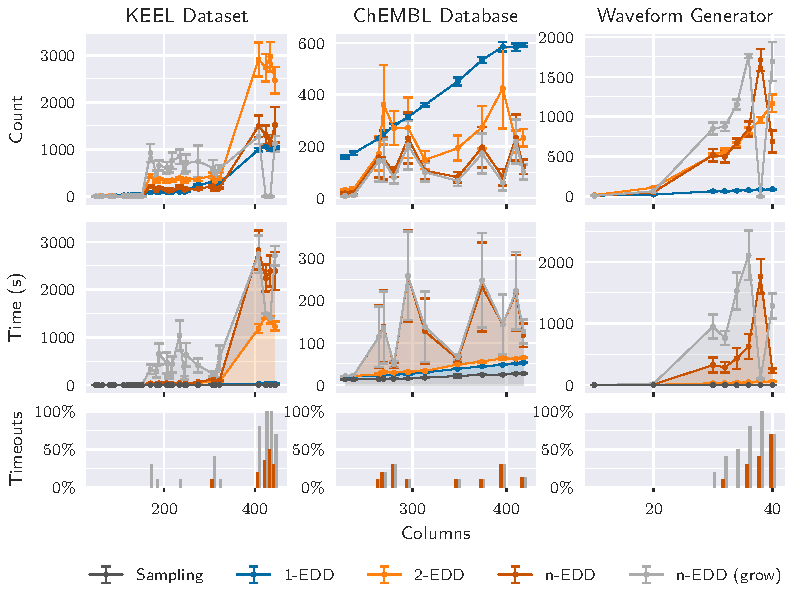
\includegraphics{images/5_presq/scalability}
    \caption[Scalability of \PresQ with respect to the number of columns.]{
        Scalability of \PresQ with respect to the number of columns.
        The top row corresponds to the number of \glspl{EDD} with arities 1, 2, and $n \ge 3$.
        The middle row shows the time spent on each stage: sampling, searching, and testing for the different arities.
        Note that the two n-EDDs variants are stacked over the previous stages, displaying the total run-time.
        The last row shows the percentage of runs timed out at 50 minutes.
        Each data point summarizes between 10 and 13 randomized runs.
    }
    \label{fig:scalability}
\end{figure*}

\begin{figure}[htb]
    \centering
    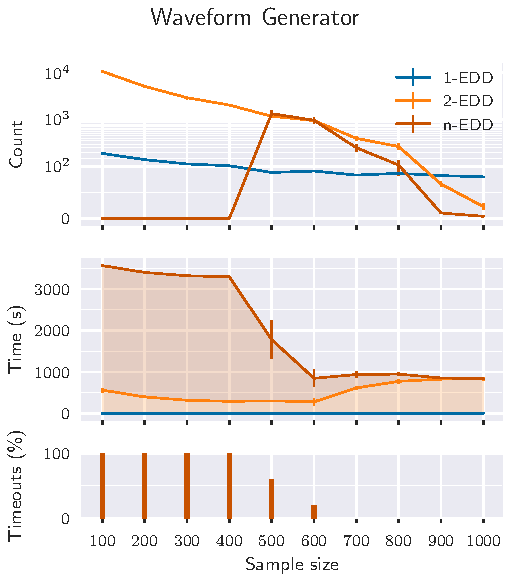
\includegraphics{images/5_presq/scalability_sample_wave}
    \caption[Scalability of \PresQ with respect to the number of samples.]{
        Scalability of \PresQ with respect to the number of samples for the Waveform datasets.
        Note that for the top row, the $y$ axis is linear between $0$ and $100$, and
        logarithmic afterward. Each data point summarizes 10 randomized runs.
    }
    \label{fig:scalability_sample_size}
\end{figure}

\FloatBarrier

\section{Conclusions}
\label{sec:presq_conclusions}

Finding sets of equally-distributed dependencies between numerical datasets is a similar
problem to that of finding Inclusion Dependencies between tables in a relational model.
However, the statistical nature of tests, with their potential uncertainties, can make
their finding more complicated and considerably degrade the performance of existing algorithms.
This problem can be mapped to finding quasi-cliques, as the \gls{IND} problem can be
mapped to finding full cliques.

In this chapter, we introduced the concept of EDD, similar to the \gls{IND} from
the relational domain. We proposed \PresQ, a new algorithm based on the search of
maximal quasi-cliques on hyper-graphs. We proved that by limiting the quasi-cliques
by the number of missing edges and the degree of the nodes, \PresQ can successfully
identify shared sets of attributes.

In general, comprehensive approaches will be needed to find very high arity \glspl{EDD},
given the complexity of the \gls{IND}/\gls{EDD} discovery problem.
In chapter~\ref{chapter:conclusions}, we discuss possible future research directions.

All the necessary code to reproduce our tests, our
measurements, and figures, are publicly available\footnote{\url{https://doi.org/10.5281/zenodo.6865856}}.
